Before presenting the results of our analysis, a brief overview of the methods used to evaluate our classification methods is needed. \\
\\
Since we are dealing with an unbalanced classification problem, the usual "accuracy" score is not suited for actually asses the quality of our classification. As said in \ref{dataset_splitting} a naive classifier that classifies every entry as "unsuccesful call" would have a \(\sim 90\%\) accuracy due to the unbalanced nature of the dataset.\\
\\
What we are really interested in is "how much our classifier outperforms randomply calling people" meaning that we are interested in a deeper analysis of our \textbf{confusion matrix}.
\\
The class we focus on is the "successful call" class, meaning that we are intrested in accuracy indicators about calls to clients that successfully subscribed to a bank account. We can introduce two measure of accuracy about our class:
\begin{description}
    \item [\(\bullet\)] the \textit{precision} is the fraction of all calls classified as succssful that are actually successful: \begin{equation}
        \text{precision} = \frac{\text{tp}}{\text{tp}+\text{fp}}
    \end{equation}
    \item[\(\bullet\)] The \textit{recall} is the fracion of all successfull calls that are correctly classified as such. \begin{equation*}
        \text{recall} = \frac{\text{tp}}{\text{tp} + \text{fn}}
    \end{equation*} 
    \item[\(\bullet\)] The \(F_1\) score is the harmonic mean of precision and recall.
\end{description}
Where \textit{tp, fp} and \textit{fn} are short for \textit{true positive, false positive} and \textit{false negative} respectively.
The above mentioned naive classifier would score \(0\) for all three measures. We will focus on the \(F_1\) score for all the tests.
\subsection{Results in Random Forests}
In experimenting with hyperparameters in Random Forest, the most impactful parameters are the one that affer to the termination criterion for each tree. In particular, the parameters \texttt{max\_depth} and \texttt{min\_sample\_leaf} are the ones that were optimized for this analysis:
\begin{description}
    \item[\(\bullet\)] \texttt{max\_depth} controls the maximum depth of each tree in the forest \\
    \item[\(\bullet\)] \texttt{min\_sample\_leaf} controls the minimum number of samples in each leaf of the trees.
\end{description}
The following code was used to search for the best parameters:

\begin{lstlisting}[language=Python, caption= Searching for the best parameters for a random forest classifier]
    from sklearn.metrics import f1_score
    from sklearn.ensemble import RandomForestClassifier

    #Searching for the best max_depth parameter
    max_depth_params = np.arange(3, 20)
    max_depth_score = []
    for d in max_depth_params:
    clf = RandomForestClassifier(max_depth=d, n_jobs=-1, random_state=42)
    clf.fit(X_train_scaled_mm, y_train)
    score = f1_score(y_true=y_test, y_pred = clf.predict(X_test_scaled_mm))
    max_depth_score.append([d, score])
    scores_md = [s[1] for s in max_depth_score]
    best_max_depth = max_depth_score[np.argmax(scores_md)][0]

    #Searching for the min_sample_leaf parameter
    min_sample_leaf_params = np.arange(1, 20)
    min_sample_leaf_score = []

    for l in min_sample_leaf_params:
    clf = RandomForestClassifier(#max_depth=best_max_depth,
                                min_samples_leaf=l,
                                n_jobs=-1,
                                random_state=42 )
    clf.fit(X_train_scaled_mm, y_train)
    score = f1_score(y_true=y_test, y_pred = clf.predict(X_test_scaled_mm))
    min_sample_leaf_score.append([l, score])
    scores_ml =  [s[1] for s in min_sample_leaf_score]
    best_min_sample_leaf = min_sample_leaf_score[np.argmax(scores_ml)][0]
\end{lstlisting}

And plotting the impact of each parameter of \(F_1\) score:

\begin{figure}[htb]
    \centering
    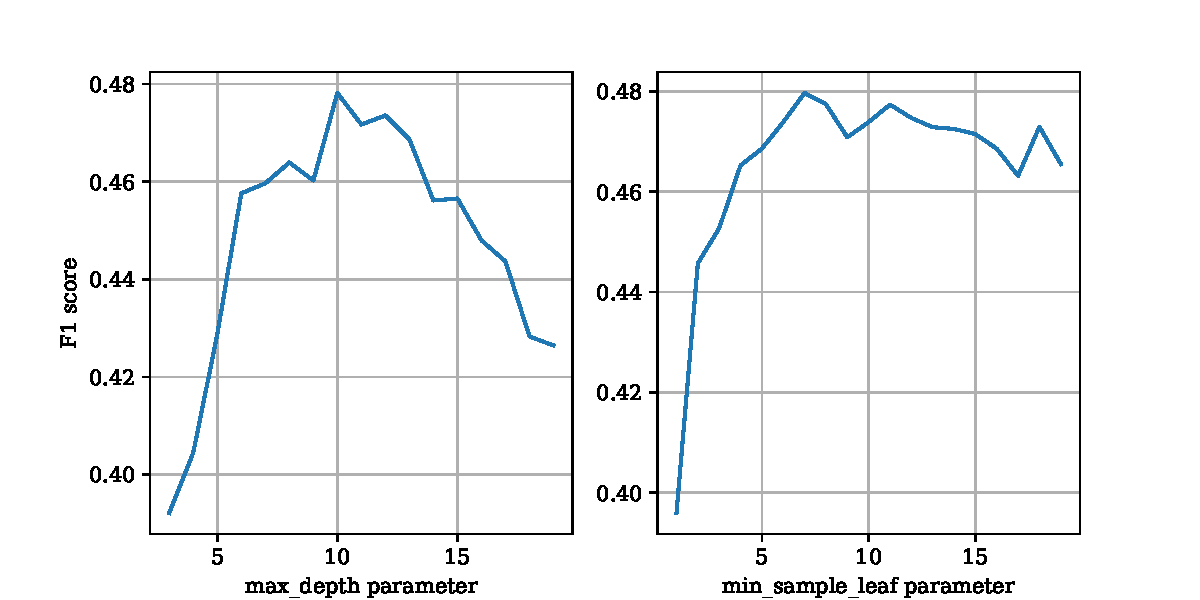
\includegraphics[scale=0.7]{pictures/random_forest_score.pdf}\
    \caption{Comparing parameters impact on \(F_1\) score on Random Forests}
    \label{fig_random_forest_score}
\end{figure}

As it is evident in figure \ref{fig_random_forest_score} we can see that the \texttt{max\_depth} parameter heavily influences the \(F_1\) score. If we then train a model using \texttt{max\_depth = 11} and \texttt{min\_sample\_leaf = 10}, we could compute the accuracy measures and the confusion matrix:

\begin{lstlisting}[language=Python, caption= Deploying the Random forest with the best parameters]
from sklearn.metrics import precision_recall_fscore_support
## Training the best random Forest
clf = RandomForestClassifier(max_depth=best_max_depth,
                             min_samples_leaf=best_min_sample_leaf, 
                             random_state=42)
clf.fit(X_train_scaled_mm, y_train)

conf_matrix = confusion_matrix(y_test, clf.predict(X_test_scaled_mm))
rf_scores = precision_recall_fscore_support(y_test,
                                            clf.predict(X_test_scaled_mm))
\end{lstlisting}
\begin{center}
    \begin{tabular}{|c|c|c|}
        \hline
        Precision & Recall & \(F_1\) score \\
        \hline
        0.30 & 0.70 & 0.41 \\
        \hline
    \end{tabular}
    \quad     
    \begin{tabular}{|c|c|c|}
        \hline
         True / Pred & Unsuccesful & Successful \\
        \hline
        Unsuccesful & 3116 & 541 \\
        \hline
        Successful & 157 & 305\\
        \hline
    \end{tabular}
\end{center}
\subsection{Results in Logistic Regression}
Logistic regression in the binary case does not have much hyperparameters to experiment with. In solving the likelyhood maximization problem we can choose to use whether an \(l_1\) or \(l_2\) norm, but through experimentation this parameter does not affect results. \\
What instead affect the accuracy is whether we use the PCA transformed dataset as training data or not. Not only computation with PCA reduced data are faster but also more accurate. 

\begin{lstlisting}[language=Python, caption= Deploying logistic regression]
from sklearn.linear_model import LogisticRegression

clf = LogisticRegression(random_state=42, solver='liblinear')
clf.fit(X_train_scaled_mm_pca, y_train)

conf_matrix = confusion_matrix(y_test, clf.predict(X_test_scaled_mm_pca))
rf_scores = precision_recall_fscore_support(y_test,
                                            clf.predict(X_test_scaled_mm_pca))
\end{lstlisting}
Deploying the above mentioned code yeld the following accuracy results:
\begin{center}
    \begin{tabular}{|c|c|c|}
        \hline
        Precision & Recall & \(F_1\) score \\
        \hline
        0.30 & 0.70 & 0.42 \\
        \hline
    \end{tabular}
    \quad     
    \begin{tabular}{|c|c|c|}
        \hline
         True / Pred & Unsuccesful & Successful \\
        \hline
        Unsuccesful & 2896 & 761 \\
        \hline
        Successful & 140 & 322\\
        \hline
    \end{tabular}
\end{center}
